\documentclass[conference]{IEEEtran}
\IEEEoverridecommandlockouts
% The preceding line is only needed to identify funding in the first footnote. If that is unneeded, please comment it out.

\usepackage{amsmath,amssymb,amsfonts}
\usepackage{algorithmic}
\usepackage{graphicx}
\usepackage{textcomp}
\usepackage{xcolor}

\usepackage{enumerate}% http://ctan.org/pkg/enumerate

\usepackage[utf8]{inputenc}

\usepackage[sorting=none]{biblatex}
\addbibresource{ref.bib}

\begin{document}

\title{Bangla Handwritten Digit Recognition\\


}


\author{\IEEEauthorblockN{Ahmad Umar Mahdi}
\IEEEauthorblockA{\textit{Department of CSE} \\
\textit{Daffodil  Intl. University}\\
Dhaka, Bangladesh \\
ahmad15-1071@diu.edu.bd}
\and
\IEEEauthorblockN{Bristy Saha}
\IEEEauthorblockA{\textit{Department of CSE} \\
\textit{Daffodil Intl.. University}\\
Dhaka, Bangladesh  \\
bristy15-1077@diu.edu.bd}
\and

\IEEEauthorblockN{Jannat Ara Shormee}
\IEEEauthorblockA{\textit{Department of CSE} \\
\textit{Daffodil Intl.. University}\\
Dhaka, Bangladesh  \\
jannat15-1080@diu.edu.bd}
\and

\IEEEauthorblockN{Shoaba Razzak}
\IEEEauthorblockA{\textit{Department of CSE} \\
\textit{Daffodil Intl.. University}\\
Dhaka, Bangladesh \\
shoaba15-2958@diu.edu.bd}

}

\maketitle

\begin{abstract}
Handwritten digit recognition is a technique for automatically recognizing and detecting handwritten digital data via Machine Learning models. To meet the demand for paperless offices and to greatly improve work efficiency, a proper Bangla handwritten digit recognition system needs to be researched and implemented. It is not easy to recognize Bengali handwritten digits due to differences in shape, size and writing style. In this paper, we used TensorFlow’s CNN Algorithm- ‘Keras Sequential Model API’ to recognize the Bangla handwritten digit. We used 6 layers in modeling. We were able to get 99.1\% accuracy in the 7th approach in recognizing Bangla handwritten digits.


\end{abstract}


\section{Introduction}
Handwritten digital recognition development research is rapidly evolving and redesigning automation fields such as automatic check reading, automatic number plate reading, digital postal service, optical image recognition (OCR), etc. Due to the different aspects of its use, computer vision researchers really feel the need to work on and improve on it - actually quality and performance. But handwriting identification is more challenging than typed letters. Because different people write differently and that creates a high level of diversity in the writing style. Also, there are some similarities between the shapes of the different characters. Overwriting situations make it even more challenging to properly classify handwritten numbers. 

Nowadays, deep learning, especially the evolutionary neural network, is doing a better job of categorizing this type of recognition work than other machine learning methods. 

The Bengali alphabet integrates the Bengali language writing system with the Assamese alphabet. Bengali is the fifth most written language in the world. With 250 million speakers, Bengali is the seventh most spoken language in the world in terms of population. Also, it is one of the major languages of the Indian subcontinent and it is the first language of Bangladesh. But compared to other languages like English, Arabic, Hindi, Chinese etc., there is very little research on Bengali handwriting recognition. 

A human brain can easily interpret a sophisticated image and can extract data from it, but for a computer, an image is a collection of pixels which are nothing but a list of combinations of numbers ranging from 0 to 255, blends being RGB, B.W., greyscale, etc. Information in an image can be extracted from the pixel values. A human eye contains light-sensitive cells that can segment the image into partitions which help to interpret the information like shape, size, and color which are called features, these features are later sent to the visual cortex that analyzes the characteristics and maps it to our memory for identification. Thus our brain is capable of identifying an unseen image. Machine learning also works like that and there are many applications that can use this Bangla Digit Recognition System. Such as Bangla Handwritten Letters Base OCR (Optical Character Recognition), Picture to Text to Speech, Bangla ID Card Reading, Number Plate Reading, Vehicle Tracking, Post Office Automation etc. And we are using the database from BHaND. Which is similar to MNIST's English handwritten digit database. So, the work will be easier. 

Our contributions - 
\begin{itemize}

\item Collecting Data
\item Pre-processing the data
\item Applying CNN with Keras API 
\item Creating Model
\item Testing the model with real life data

\end{itemize}

\section{Research Aims}
The goal of this investigation is to build up a superior Bangla Handwritten Digital Recognition System. Our aim is to achieve the accuracy as best as possible in recognizing Bangla Handwritten Digit.


\section{Literature Review}

The most common reference for a multi-layer perceptron is 90.37. Deep Neural also later promised a solid handwriting solution in which case the TDNN model is also used to convert handwritten numbers (FNDN) using the (CNN) model. Many machine learning solutions have been created for different solutions. It is very difficult to read the handwritten numbers of different pictures. CNN is later used as DCNN for handwriting. 96.25\% and 96.99\% of the two models of the neuron model (FRDNN) are more than 100, respectively. But the FRDNN model network is more powerful than TDNN for writing Yug Bangla. Friendly recognition in the proposed method indicates fair calculation. \cite{Hossain2021-ns} 

In 1959 Grimsdale made an initial significant attempt at character identification research. Of great importance in Eden's work was the fact that he formally proved that all manuscripts were composed of a limited number of planned features, a point which had previously been implicitly included. This concept at work was later used in all methods in the syntactic method of character identification. The goal of this project is to implement a classification algorithm for identifying handwritten numbers. Probably the most widely used machine learning algorithms, such as SVM, KNN, and RFC, and the after-effects of deep learning calculations, such as multilayer CNN using kerosene with Thiago and TensorFlow. Using these, 98.70\% accuracy uses CNN while 97.91\% uses SVM, 96.67\% uses KNN, and 96.89\% uses RFC. \cite{Siddique2019-ku} 

Their proposed method has achieved 98.51\% accuracy for real-world handwritten number prediction and has lost less than 0.1\%. Since the loading dataset is necessary for any process, all the steps come after it. Our model is designed to work with real-world data, and real-world images are not even close to MNIST raster images, with a lot of pre-processing to make a real image look like a raster image. CNN's performance for handwritten recognition has been significant. The proposed method achieves 98\% accuracy and is also able to detect real-world images, with a loss percentage of less than 0.1 in both training and evaluation, which is negligible. \cite{Bharadwaj2020-wf} 



\section{Research Question}
\begin{enumerate}
  \item How is Keras related to TensorFlow? \\ {\small Ans: TensorFlow is an open-sourced end-to-end platform, a library for multiple machine learning tasks, while Keras is a high-level neural network library that runs on top of TensorFlow.}

  \item What data is used to train and test the machine learning methods?\\ {\small Ans: We are using the BHaND Dataset which contains 70000 Handwritten Bangla Digits.}
\end{enumerate}


\section{Research Objectives}
\begin{itemize}
  \item To learn about image processing in Python.
  \item To learn applying Machine Learning Algorithms in image.
  \item To build something that is really helpful for the current generation.
  \item Achieving best accuracy in recognizing Bangla handwritten digits. 
\end{itemize}


\section{Research Methodology} 
Our proposed method is mainly separated into three stages. Those are-
\begin{enumerate}[ A.]
  \item Dataset Description 
  \item Data Preprocessing
  \item Model Training
\end{enumerate}

\subsection{Dataset Description}
In this paper, we used the BHaND dataset \cite{saadat2016b} from GitHub as a primary dataset to train the model which contains 70000 handwritten Bangla digits. From which 50000 digits are used for training and validation. 20000 digits are used for testing. BHaND data is represented in the png file format and looks like in ``Fig.~\ref{fig1}''. The images are gray-scale and the dimension is 32 × 32. Each row of these sets has two dimensions, the first dimension is the image itself and the second dimension is the label. Here the label means which digit (0 to 9 in Bengali) this image represents. Thus the training set has 50,000 rows and two columns. Other sets are also similar in nature. 

\begin{figure}[htbp]
\centerline{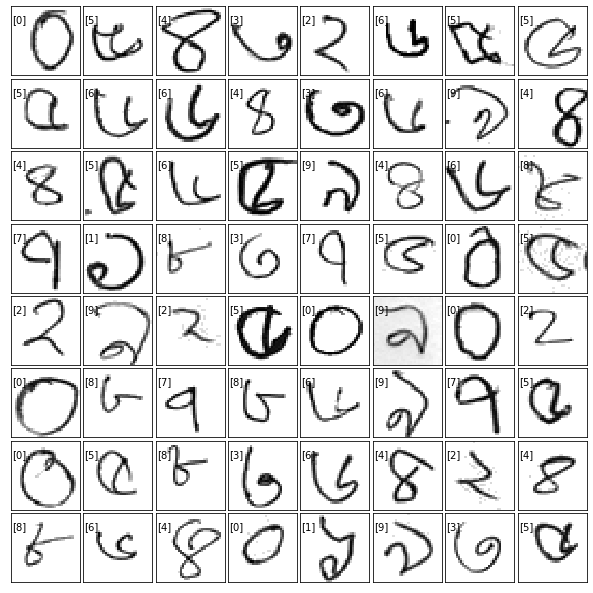
\includegraphics[scale=.4]{fig1.png}}
\caption{Dataset Visualization}
\label{fig1}
\end{figure}

Each of the samples are in gray-scale form normalized to the intensity range [0,1] and the intensity were inverted to make black pixels 1 and white pixels 0. The images were then reshaped to a single dimension making 1024 (32*32) features in total ``Fig.~\ref{fig2}''. Thus the first dimension of each row in each set is a 1024 dimension vector and the second dimension of each row in each dataset is a regular integer number (0 to 9).

All these samples were then grouped together in a single pickle file using python's serializer Pickle, then they were compressed by GZIP compression algorithm for faster transmission.

\begin{figure}[htbp]
\centerline{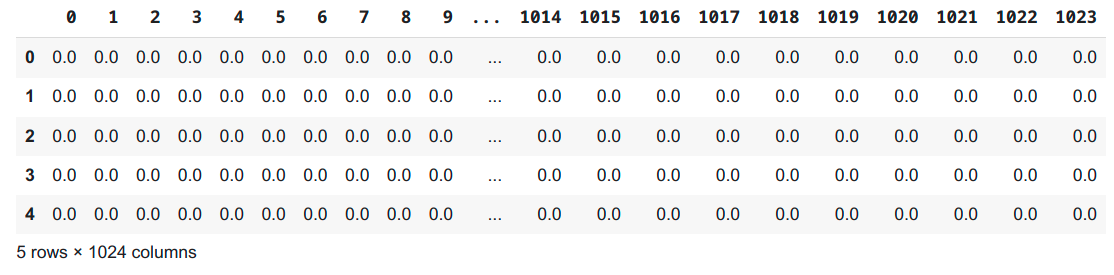
\includegraphics[scale=.3]{fig2.png}}
\caption{DataFrame}
\label{fig2}
\end{figure}

\subsection{Data Preprocessing}
First we have to invert the image so that black pixels are close to 1 and the white pixels are close to 0.  Then we have to normalize the image by converting values that are less than 0.5 to 0. Then we can crop the extra background to get better results. Now we shape the data to our required square shape 32x32 ``Fig.~\ref{fig2}''. Now, we have to compress the data to a GZIP file to use it easily in our project.

\begin{figure}[htbp]
\centerline{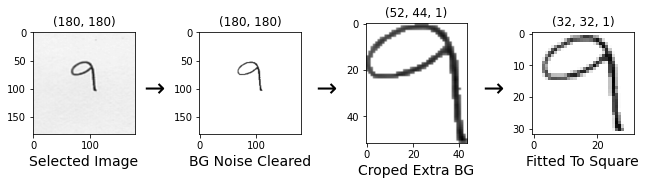
\includegraphics[scale=.4]{fig3.png}}
\caption{Preprocessing}
\label{fig3}
\end{figure}

Now we load that GZIP compressed file in our project and we decompress the file. After decompressing we load the pickle file to three two dimensional Tuple sets (trainSet, validSet, testSet). Then we separate that tuple to (X\_train, y\_train) Arrays. Here, X\_train is our png data and y\_train is our label of that data. Then we convert those two Arrays to Pandas DataFrame. We do similar operations for validSet and testSet. 

Now, we have to reshape our data by transforming X\_train sets from a 50000x1024 dataframe to a 50000x32x32x1 4D tensor for Keras modeling. Here, we have 50000 images in the train set which are in 32x32 pixels and the 4\textsuperscript{th} dimension is for color profile. Our color profile is 1 means those are gray-scale images.\\ 


\subsection{Model training}

To train our model we used Sequential Modeling. A Sequential model is appropriate for a plain stack of layers where each layer has exactly one input tensor and one output tensor. It is a way of creating deep learning models where an instance of the Sequential class is created and model layers are created and added to it.\\

We used 5 types of layers in our Model.\\Those are-

\begin{enumerate}
  \item \textbf{Conv2D:} Keras Conv2D is a 2D Convolution layer. This creates a convolution kernel that is wind with layers input which helps produce a tensor of outputs. The most common type of convolution that is used is the 2D convolution layer.
  \item \textbf{MaxPool2D:} Max pooling operation for 2D spatial data. Downsamples the input along its spatial dimensions (height and width) by taking the maximum value over an input window (of size defined by pool\_size) for each channel of the input.
  \item \textbf{Flatten:} It flattens the multi-dimensional input tensors into a single dimension, so you can model your input layer and build your neural network model, then pass those data into every single neuron of the model effectively.
  \item \textbf{Dense:} Dense layer is the regular deeply connected neural network layer. Each neuron in the dense layer receives input from all neurons of its previous layer. It is the most common and frequently used layer.
  \item \textbf{Dropout:} The Dropout layer randomly sets input units to 0 with a frequency of rate at each step during training time, which helps prevent overfitting.
\end{enumerate}

Here is our Model Summary:
\begin{figure}[htbp]
\centerline{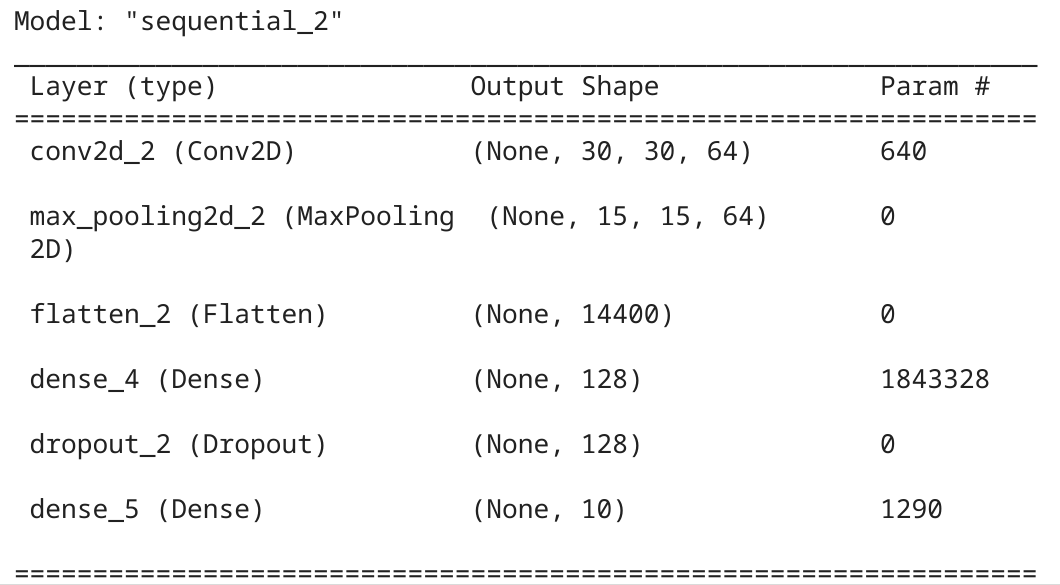
\includegraphics[scale=.3]{fig4.png}}
\caption{Model}
\label{fig4}
\end{figure}

\section{Result}

We were able to get 99.1\% accuracy after 7 Eproch in Model fitting. Model fitting is a measure of how well a machine learning model generalizes to similar data to that on which it was trained.

\begin{figure}[htbp]
\centerline{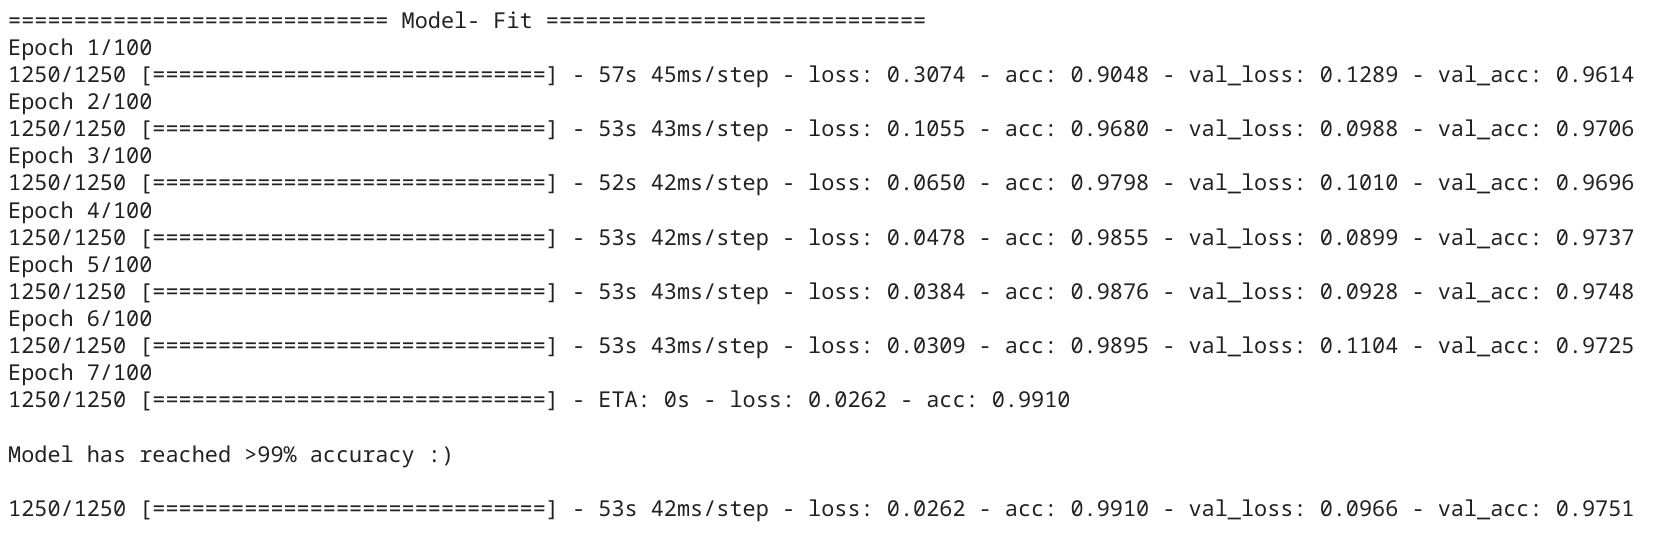
\includegraphics[scale=.2]{fig5.png}}
\caption{Model-Fit}
\label{fig5}
\end{figure}

We also can visualize our accuracy and loss by showing the Confusion Matrix. Here is our Confusion Matrix:


\begin{figure}[htbp]
\centerline{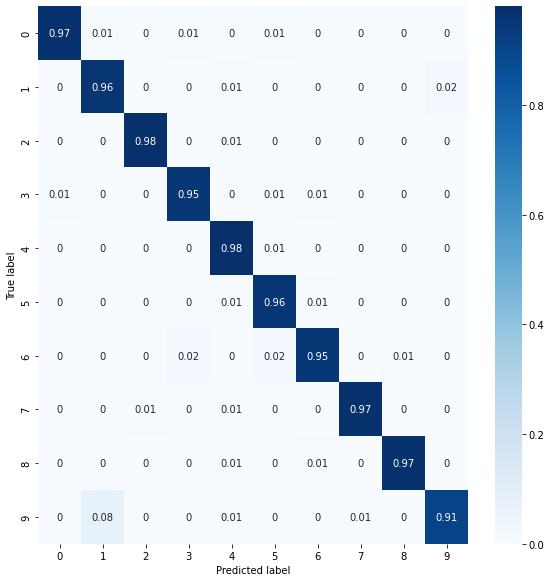
\includegraphics[scale=.39]{fig6.png}}
\caption{Confusion Matrix}
\label{fig6}
\end{figure}


\section{Conclusion}
In this research, we proposed to use deep learning approaches for handwritten Bangla digit recognition for lesser epochs and less computation time. We evaluated the performance of Keras Modeling. Among some of the observations, the maximum accuracy in the performance was found to be 99.1%. Research work is currently progressing to develop more.


\printbibliography

\end{document}
